\newpage
\section{Teoria}
\subsection{Osciladores}
Osciladores podem, geralmente, ser categorizados como amplificadores com feedback positivo ou como circuitos de resistência negativa, sendo que, neste laboratório será analisado os circuitos com feedback positivo.

\subsection{Ganho do amplificador realimentado}
A figura \ref{f_gain} mostra o diagrama de bloco que representa um amplificador genérico ligado com feedback positivo.
Neste tipo de amplificador o sinal de entrada $X_s(t)$ é somado ao sinal de saída $X_0(t)$ multiplicado por um ganho $\beta$. Sendo assim, temos que o ganho de transferência do amplificador é 
\[
A_f = \frac{X_0}{X_s} = \frac{A}{1+\beta A}.
\]

Sendo que, para que haja oscilação, o sinal $X_f$ deve estar com uma defasagem de 0 graus em relação a $X_i$. Isto pode ser obtido colocando um bloco de atraso entre $X_s$ e $X_i$.

\begin{figure}[H]
\centering
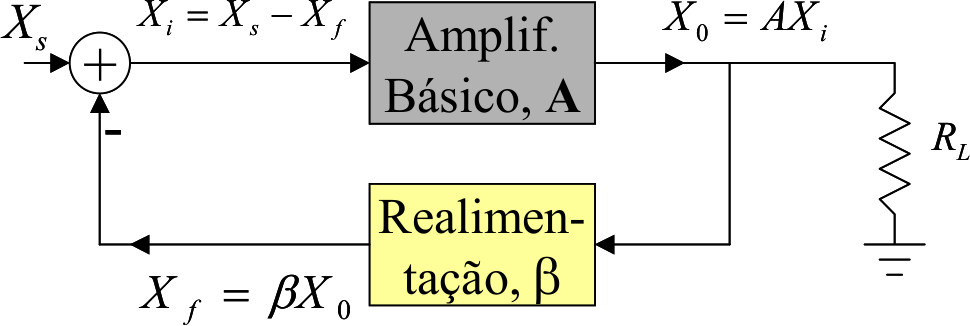
\includegraphics[scale=0.5]{Imagens/gain.png}
\caption{Diagrama de blocos de um amplificador com realimentação positiva.}
\label{f_gain}
\end{figure}

Um outro fator é para que haja oscilação é que $1+A\beta = 0$, ou seja $A\beta = -1$.
Como os componentes envolvidos não são ideais, calcula-se o ganho $A\beta$ para valores entre $-1.05$ a $-1.20$.

A frequência de oscilação do circuito (dado que os critérios acima são respeitados), para osciladores a cristal, é determinada pela frequência de resonância do cristal de quartzo.

